\chapter{Choosing a Prediction Model}
\thispagestyle{nohead}
\label{Prediction}

This chapter will evaluate the effectiveness of a number of machine learning algorithms at predicting the most appropriate SMT solver to use on any (unseen) \why~PO.
Our goal in this thesis is to construct a ``meta-solver'' or \textit{portfolio} solver which chooses from a range of tools in order to prove more goals than a single solver is capable of.
We motivate the need for a portfolio solver with an analysis of our dataset 
in Sec. \ref{sec:portfolio-benefit}. 
More details about the type of prediction task chosen for the evaluation of ML algorithms is given in Sec. \ref{sec:reg-class}, with an introduction to a number of theoretical and practical strategies chosen for comparison in Sec. \ref{sec:theoretical} and \ref{sec:practical}. A more detailed introduction to the six prediction models (introduced previously in Sec. \ref{sub:lrsvmmml} and Table \ref{table:algorithms}) is given in Sec. \ref{pred:choosing} before the results of their comparison is discussed. We end this chapter with a more detailed look at the model chosen for use in the actual implementation of \where~.

\section{The benefit of portfolio-solving in \why}
\label{sec:portfolio-benefit}

\newcolumntype{Z}{>{\raggedleft\arraybackslash}X} 
\begin{table}
	\caption[Results of running 8 solvers on the example \why~programs]{Results of running 8 solvers on the example \why~programs.  Also included is a theoretical solver  $ \mathcal{TS}$, which always returns the best answer in the fastest time.}
	\begin{tabularx}{1.1\textwidth}{@{}l|ZZZ|ZZZ|ZZZ@{}}
		\toprule
		{} & \multicolumn{3}{c|}{\textbf{File}} & \multicolumn{3}{c|}{\textbf{Theory}} & \multicolumn{3}{c}{\textbf{Goal}} \\
		{} & \# proved & \% proved & Avg time & \# proved & \% proved & Avg time & \# proved & \% proved & Avg time \\
		\midrule
		$ \mathcal{TS}$ & \textbf{48} & \textbf{37.5\%} & \textbf{1.90} & \textbf{190} & \textbf{63.8\%} & \textbf{1.03} & \textbf{837} & \textbf{79.9\%} & \textbf{0.42} \\
		\textbf{Alt-Ergo-0.95.2} & 25 & 19.5\% & 1.45 & 118 & 39.6\%& 0.77 & 568 & 54.2\% & 0.54 \\ 
		\textbf{Alt-Ergo-1.01} & 34 & 26.6\% & 1.70 & 142 & 47.7\% & 0.79 & 632 & 60.3\% & 0.48 \\ 
		\textbf{CVC3} & 19 & 14.8\% & 1.06 & 128 & 43.0\% & 0.65 & 597 & 57.0\% & 0.49 \\ 
		\textbf{CVC4} & 19  & 14.8\% & 1.09 & 117 & 39.3\% & 0.51 & 612 & 58.4\% & 0.37 \\ 
		\textbf{veriT} & 5 & 4.0\% & 0.12 & 79 & 26.5\% & 0.20 & 333 & 31.8\% & 0.26 \\ 
		\textbf{Yices} & 14 & 10.9\% & 0.53 & 102 & 34.2\% & 0.22 & 368 & 35.1\% & 0.22 \\ 
		\textbf{Z3-4.3.2} & 25 & 19.5\% & 0.56 & 128 & 43.0\% & 0.36 & 588 & 56.1\% & 0.38 \\ 
		\textbf{Z3-4.4.1} & 26 & 20.3\% & 0.58 & 130 & 43.6\% & 0.40 & 581 & 55.4\% & 0.35 \\ 
		\bottomrule
	\end{tabularx}
	\label{table:avgtimes}
\end{table} 


Now that the SMT solvers to be supported by \where~have been identified and an appropriate dataset for training and testing purposes has been chosen, we can make a preliminary and exploratory analysis of the behaviour of the SMT tools on the particular data. 
We aim to make a case for portfolio-solving as an effective method for discharging POs in the \why~system.

We refer the reader to Table \ref{table:avgtimes} which shows the results of running 8 solvers on the example \why~programs with a timeout value of 10 seconds. 
The entire dataset is used in this case. 
WhyML files are modularised as a number of \textit{theories}. The \why~IVL identifies the \textit{goals} which need to be proven in order for the theory (and in turn the entire file) to be verified as correct. 
Our dataset of 128 WhyML files consists of 289 theories, which in turn generate 1048 goals. 
Aside from the number of each modular construct proved by the solver (left sub-column), the percentage this number represents of the total is given (centre sub-column) and the average time taken to prove each construct (as measured using the process described in Sec. \ref{sub:confidence}) is given in the right sub-column. 

Table \ref{table:avgtimes} also shows the results for a \underline{T}heoretical \underline{S}olver $ \mathcal{TS} $. 
$ \mathcal{TS} $ is the best solver, from the eight SMT solvers measured, chosen on a per-goal basis. 
For example, if a file contains one theory which consists of three goals, and the best-performing solver is CVC4 for the first goal, Yices for the second, and CVC3 for the third, the result for $\mathcal{TS}$ on that file is the sum of the results for CVC4 on the first goal, Yices on the second, etc.
We define what is means for a solver to be the \textit{best} in the next subsection.

It is important not to confuse $\mathcal{TS}$ with the theoretical \textsf{Best} ranking introduced in Sec. \ref{sec:strategies}. 
$\mathcal{TS}$ refers to a single solver (and hence is directly comparable to the other eight SMT solvers in Table \ref{table:avgtimes}), while \textsf{Best} refers to a \textit{ranking} which uses all eight solvers\footnote{$\mathcal{TS}$ is, in fact, the result of using the top-ranking solver from \textsf{Best} and stopping.}.


The theoretical solver $\mathcal{TS}$ shows the benefit of being able to use the most appropriate solver for each PO: 205 more goals are provable --- an increase of 19.6\% --- over the best single solver (Alt-Ergo version 1.01). 

\subsection{The relative utility of solver responses}

To make assertions about the relative performance of different solvers on the same goal, a definition of the relative \textit{utility} of solver responses is required.
Should a solver that returns an answer of \textit{Valid} in 5 seconds be seen as ``worse'' than one that returns \textit{Unknown} in 0.5 seconds? 
Likewise, should the solver returning \textit{Failure} after 1 second be penalised more severely than one returning \textit{Timeout} after the maximum time limit?

We define a total ordering for response utility as 
\[
Valid > Invalid > Unknown > Timeout > Failure
\]  
the reasoning being that a \textit{Failure} response usually signals a fatal error in the logic encoding for that solver/goal pair, and the learning algorithm should be discouraged from choosing a failing solver for the particular goal characteristics in question. 
As discussed in Sec. \ref{sub:timeout-limit} of the previous chapter, \textit{Unknown} answers are returned quickly in general, and should not be penalised as much as \textit{Timeout} responses. 
Solvers which reach the timeout limit are unlikely to return a \textit{Valid} or \textit{Invalid} response give more time (illustrated clearly by Fig. \ref{fig:line_graph}).
Solvers returning the same answer are ranked according to runtime --- with faster solvers being preferred.

This method for defining relative performance has similarities to the scoring structure for ATPs competing in SV-COMP \cite{Beyer2016, SVCOMP}, with some important differences. 
Although the notion of ``false positive'' and ``false negative'' responses is not applicable in the SMT domain, a ``true positive'' is scored marginally higher than a ``true negative''. 
In contrast, \textit{Unknown, Timeout} and \textit{Failure} responses are not treated separately by the SV-COMP model --- they all fall under the \textit{Unknown} response category and receive a score of zero.

A further refinement to our scoring model was necessary in order for the prediction models to operate effectively. 
The definition of the \textit{cost} function we applied to solver results is given in Sec. \ref{sub:scoring} of this chapter. 

\section{Classification and regression}
\label{sec:reg-class}

Machine learning prediction tasks can be separated into two categories: those involving the \textit{classification} of a variable into discrete categories or classes, and those predicting a continuous-valued variable directly --- \textit{regression} tasks.
This section will discuss some of the options considered when designing \where's prediction task.

\subsection{Predicting the single best solver} This option involves a multi-class classification task: the classes involved are the eight SMT solvers.
Each PO is classified as belonging in one class. 
This direction was rejected as some benefits associated with portfolio-solving were lost: if the PO is misclassified, the performance of the portfolio solver suffers severely.
\subsection{Predicting the best \textit{ranking} of solvers} Again, this option is a multi-class classification task. 
Instead of predicting a single solver, however, the task involves predicting the entire ranking of eight solvers. 
The benefit of obtaining a ranking is the flexibility it affords in calling SMT solvers sequentially or in parallel.
If the first solver fails or is mispredicted as being the best, the next best predicted solver is called, and so on.
With 8 SMT solvers there are 8! rankings --- far too many to be reasonable for a classification task --- leading to this approach being rejected.
There were no examples of many possible rankings in the training data - making the prediction of such rankings on unseen instances impossible.
\subsection{Predicting solver runtime and response separately}
This approach involves two separate tasks, each predicting a characteristic of the solver's performance. 
One algorithm would attempt to predict the response class (i.e. \textit{Valid, Invalid}, etc.) while another would attempt to predict the solver runtime.
The former task is a multi-class classification task with five classes, while the latter is a regression task.
This method has the advantage of affording the user flexibility in how to choose the ultimate ranking: if fast responses are preferred over \textit{Valid} answers.
This flexibility comes at the price of complexity, however: two accurate predictors, a classifier and regressor, are required instead of one.
\subsection{Combining the prediction of solver response and runtime}
This option uses a cost function to combine the two solver response variables as a single real-valued number which is used for ranking the solvers.
Using this method,  

\subsection{The Cost Function}
\label{sub:scoring}
%maybe leave until it is fixed

\section{Ranking strategies}
\label{sec:strategies}

The following ranking strategies provide a basis by which we can compare 

\subsection{Theoretical \textsf{Best}}
\subsection{Theoretical \textsf{Random}}
\subsection{Theoretical \textsf{Worst}}
\subsection{\textsf{Fixed}}

\section{Choosing the most effective algorithm}
\label{pred:choosing}
\begin{figure}
	\centering
	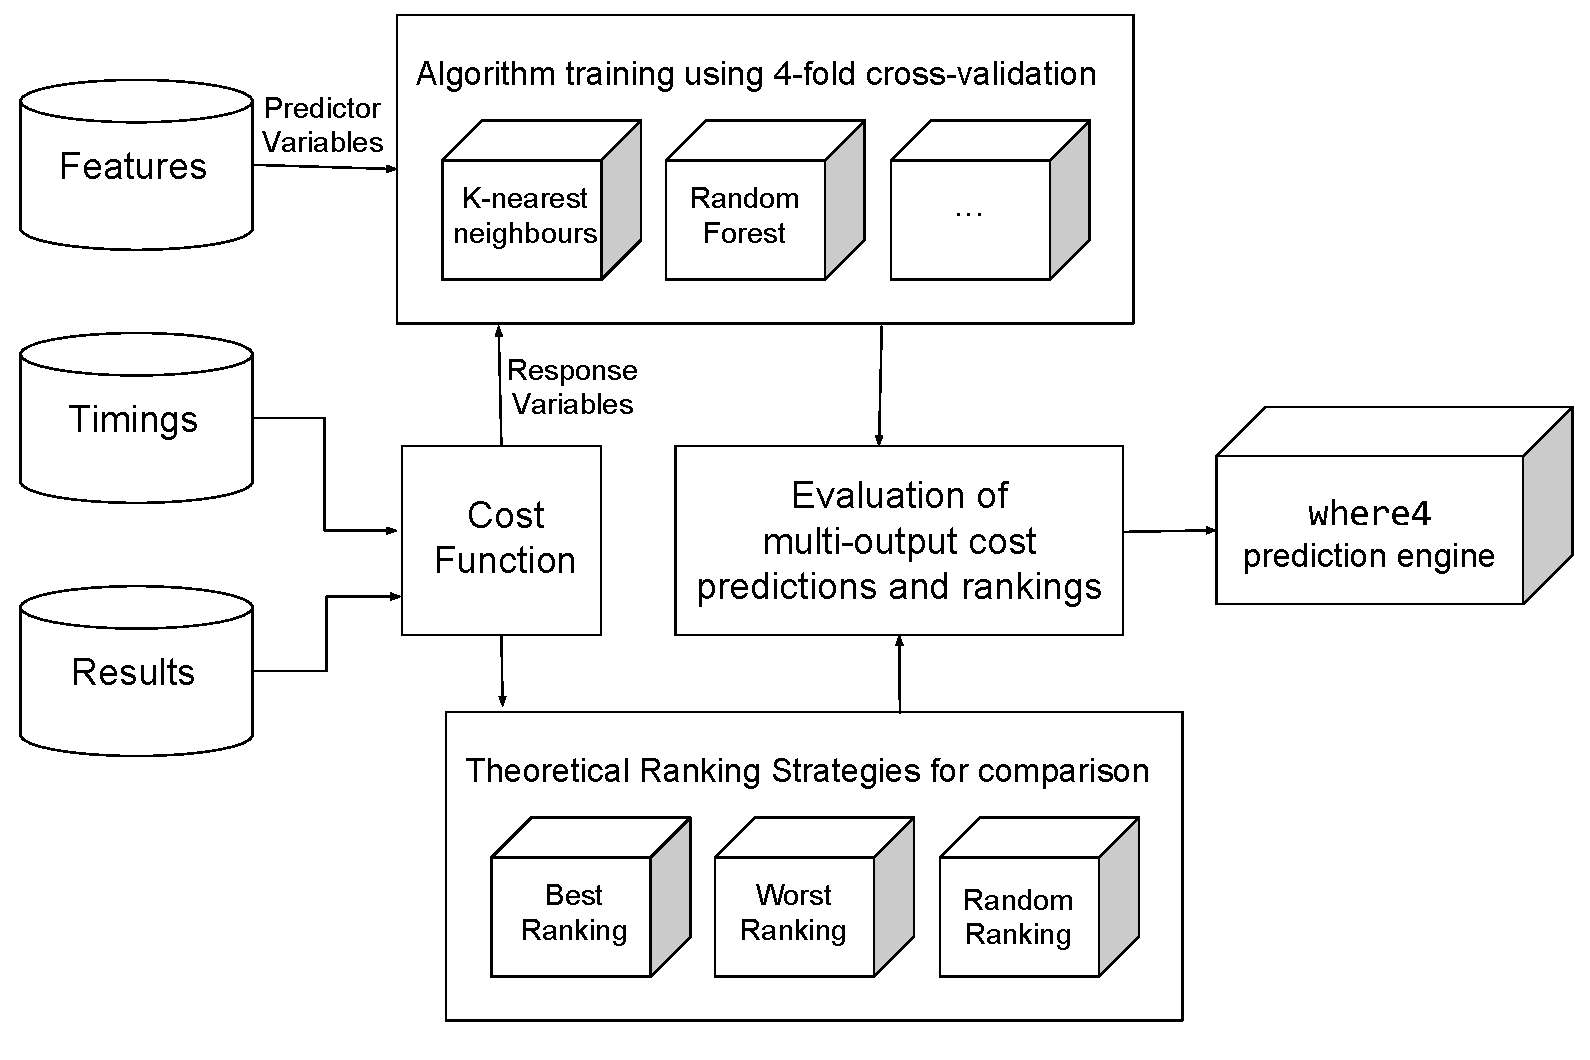
\includegraphics[width=0.9\linewidth]{Figures/Chapter4}
	\caption{Overview of the process used to derive the \where~prediction model}
	\label{fig:Chapter4}
\end{figure}

\subsection{Train / Test Split}
\subsection{Instance Weighting}
\subsection{Normalised Distributed Cumulative Gain}
\subsection{Mean Average Error}
%\subsection{The prediction of score as a regression task}
%\subsection{The prediction of \textit{result} as a classification task}
%\subsection{The prediction of \textit{time} as a regression task}
%\subsection{The prediction of \textit{time} as a classification task}
%\subsubsection{Binarization}
%\subsubsection{Multiclass via binning}
%\subsection{The prediction of score as an ensemble task}
%\subsection{The prediction of score as a multi-label task} 
\subsection{Properties of multi-output problems}
\label{sub:multi}

\section{The chosen model}
\label{sec:chosen}

